

\chapter{Stand der Wissenschaft und Technik}\label{cha:2}

Zur Abbildung geeigneter Welleneigeschaften in einer Messkabine, die selbst ebenfalls möglichst wenig Beeinflussung durch äußere Felder erfährt, ist ein grundlegendes Verständnis elektrischer und magnetischer Felder, sowie deren Ausbreitung im Raum und Interaktion mit unterschiedlichen Grenzschichten notwendig. Weiterhin soll die Schirmdämpfung als zu messende Größe der CNT-Folien allgemein betrachtet werden, sodass im Anschluss daran verschiedene Möglichkeiten der Messung vorgestellt werden können. \par
\vspace{\linespace}
Mithilfe der Theorie der Eigenschaften von Wellenfeldern wird dann aus betrachteten Messmethoden die ausgewählt, mit der sich die Anforderungen an die durchzuführende Vermessung von Schirmmaterialien bestmöglich erfüllen lassen. Die wissenschaftlichen Grundlagen dienen weiterhin als Basis für die Detailkonstruktion der Messkabine.


\section{Grundlagen elektromagenetischer Wellenfelder}\label{cha:2_Grundlagen}


Allgemein beschreibt ein Feld die Gesamtmenge aller Werte einer physikalischen Größe, die allen Punkten eines leeren oder stoffgefüllten Raumes zugeordnet sind, die sogenannte Feldgröße \cite{Spektrum.de_Feld}. Je nach Art der Feldgröße wird der allgemeine Feldbegriff in Skalarfeld 

\begin{equation}
    a(x,y,z, \ldots)    
\end{equation}


und Vektorfeld 

\begin{equation}
    \vec A(x,y,z,\ldots)
\end{equation}

unterteilt. Durch die Darstellung der Abhängigkeit von den Ortskoordinaten des Raumes wird deutlich, dass es sich bei einer Größe um ein Feld handelt. \par
\vspace{\linespace}
Die im Rahmen dieser Arbeit wichtigen Felder sind das elektrische und das magnetische Feld. Eine Beschreibung des Zusammenhanges zwischen der Feldursache und dem entstehenden Feld lässt sich in beiden Fällen mithilfe der Materialgleichungen und der Maxwell'schen Gleichungen vornehmen~\cite{EM_Schirmung}. Grundlegend lässt sich ein Feld jedoch auch ohne Kenntnis seiner Ursache beschreiben, sodass im Rahmen dieser Arbeit nicht explizit auf die Maxwell'schen Gleichungen eingegangen werden soll, da dies thematisch zu weit führen würde. 


\subsection{Elektrisches Feld}\label{cha:2_sub_Elektrisches_Feld}

Um das elektrische Feld mittels seiner Wirkungs zu beschreiben, wird eine Testladung in das Feld eingebracht, auf die daraufhin eine Kraft $\vec F_q(x,y,z,q)$ wirkt. Da die Kraft eine gerichtete Größe ist, muss die Beschreibung des elektrischen Feldes mittels eines Vektorfeldes beschrieben werden. Die Größe der Kraft ist abhängig von der eingebrachten Ladung. Um eine Veränderung des Feldes durch die Testladung auszuschließen, wird stattdessen eine infinitesimale Teilladung $dq$ zur Beschreibung des Feldes verwendet, was sich damit aus

\begin{equation}
    \vec E (x,y,z) = \frac{d\vec F_q(x,y,z,q)}{dq}
\end{equation}

ergibt. Der Differentialquotient $\vec E$ ist die elektrische Feldstärke \cite{EM_Schirmung}. \par
\vspace{\linespace}
Damit ist die Wirkung eines elektrischen Feldes beschrieben, jedoch noch nicht dessen Ursache. Nach dem sogenannten Satz des Hüllenflusses, dem ersten Maxwell'schen Gesetz, erfahren Ladungen nicht nur Beeinflussung durch ein elektrisches Feld, sondern sind auch dessen Ursache. Eine Beschreibung kann am einfachsten mithilfe eines Plattenkondensators erfolgen, dessen Plattenflächen $A_P$ senkrecht auf den Feldlinien eines elektrisches Feldes stehen und auf welche die Ladungen $+q$ und $-q$ genau so aufgebracht werden, dass im Inneren des Kondensators das äußere Feld kompensiert wird. Eine von der Fläche unabhängige Größe zur Beschreibung des elektrischen Feldes lässt sich wiederum durch den Differentielquotienten 

\begin{equation}
    \vec D(x,y,z) = \frac{dq}{dA_P} \cdot \vec n_A
\end{equation}

erhalten, der elektrischen Flussdichte $\vec D$ \cite{EM_Schirmung}. \par
\vspace{\linespace}

Da sowohl die Feldstärke als auch die Flussdichte das elektrische Feld beschreiben, gibt es in Abhängigkeit Materials, aus dem der felderfüllte Raum besteht, einen Zusammenhang zwischen beiden Größen, die sogenannte Dielektrizitätszahl oder Permittivität $\varepsilon$, die eine Materialeigenschaft ist. Es gilt

\begin{equation}
    \vec D = \varepsilon \cdot \vec E = \varepsilon_0 \varepsilon_r \cdot \vec E \qquad \quad \text{mit} \qquad \varepsilon_0 = 8,85419 \cdot 10^{-12} \; \si{\ampere\second\per\volt\per\meter}
    \label{eq:2_Materialgleichung_elektrisches_Feld}
\end{equation}

mit der Dielektrizitätszahl des leeren Raumes $\varepsilon_0$ und der relativen Dielektrizitätszahl $\varepsilon_r$ des betrachteten Materials \cite{EM_Schirmung}.


\subsection{Magnetisches Feld}\label{cha:2_sub_Magnetisches_Feld}

Wie auch die elektrische Feldstärke wird die magnetische Flussdichte indirekt beschrieben, d.h. über ihre messbare Kraftwirkung auf elektrische Ströme bzw. bewegte Ladungen. Dabei wird ein stromdurchflossener Draht der Länge $L$ so über einem Magnetfeld angeordnet, dass die messbare Kraft maximal wird. Um auch hier Rückwirkungen auszuschließen, wird eine differentielle Drahtlänge, die vom infinitesimal kleinen Strom $dI$ durchflossen wird, betrachtet. Mit des Differentialquotienten

\begin{equation}
    \vec B(x,y,z) = \frac{d^2 \vec F_L(x,y,z,L,I)}{dL \cdot dI}
\end{equation}

lässt sich die magentische Flussdichte, die sowohl vom Strom $I$ als auch von der Drahtlänge $L$ abhängt, aus der gemessenen Kraft ermitteln \cite{EM_Schirmung}. 
\par
\vspace{\linespace}
Analog zur Betrachtung elektrischer Felder lässt sich feststellen, dass Ströme nicht nur eine Kraftwirkung durch magnetische Felder erfahren, sondern auch deren Ursache sind. Dazu lässt sich ebenfalls ein einfaches Gedankenexperiment ähnlich der Betrachtung zur elektrischen Flussdichte durchführen: 
\par
\vspace{\linespace}
In einer Spule der Länge $L$ fließe ein Strom $I$, der genau so groß ist, dass durch die induzierte magnetische Flussdichte ein umgebendes äußeres Magnetfeld im Inneren der Spule verschwindet. Die Ausrichtung der Anordnung sei wiederum so erfolgt, dass der Strom $I$ maximal wird. Der erforderliche Strom ist abhängig von der Spulenlänge und deren Windungszahl $N_w$. Das Differential

\begin{equation}
    \vec H(x,y,z) = N_w \frac{dI(x,y,z,L)}{dL} \cdot \vec n_A
\end{equation}

beschreibt die magnetische Feldstärke, welche senkrecht auf der Spulenquerschnittsfläche steht \cite{EM_Schirmung}. 
\par
\vspace{\linespace}
Ebenso wie die elektrische Feldstärke und Flussdichte sind auch die beschreibenden Feldgrößen des magnetischen Feldes proportional zueinander und lassen sich über eine Materialkonstante, der sogenannten Permeabilität $\mu$, ineinander umrechnen:

\begin{equation}
    \vec B = \mu \cdot \vec H = \mu_0 \mu_r \cdot \vec H \qquad \quad \text{mit} \qquad \mu_0 = 4\cdot \pi \cdot 10^{-7} \; \si{\volt\second\per\ampere\per\meter}.
    \label{eq:2_Materialgleichung_magnetisches_Feld}
\end{equation}

Die relative Permeabilität $\mu_r$ ist ein Materialparameter und die Permeabilität des Vakuums $\mu_0$, ebenso wie $\varepsilon_0$, eine Naturkonstante \cite{EM_Schirmung}.
\par
\vspace{\linespace}
Eine Verknüpfung des elektrischen Feldes mit dem magnetischen kann über den ein einem Leiter hervorgerufenen Stromfluss erfolgen. Die verknüpfende Größe der erzeugten Stromdichte $\vec j$,

\begin{equation}
    \vec j = \sigma \cdot \vec E,
\end{equation}

ist dabei die Leitfähigkeit $\sigma$ des betrachteten Leitermaterials.


\subsection{Verhalten elektrischer und magnetischer Felder an Grenzflächen}

In den vorangegangenen \Abschnitten \ref{cha:2_sub_Elektrisches_Feld} und \ref{cha:2_sub_Magnetisches_Feld} wurde die Abhängigkeit der Flussdichte- und Feldstärkevektoren voneinandern mithilfe von Materialeigenschaften beschrieben. Breiten sich die Felder also entlang verschiedener Materialien mit unterschiedlichen Dielektrizitäten und Permeabilitäten aus, ändern sich beim Übergang zwangsläufig die Ausbreitungsbedingungen. Dies soll im Folgendes betrachtet werden, da das Verhalten der Felder an Materialgrenzflächen grundlegend für die Untersuchtung von Materialschirmen ist. 
\par
\vspace{\linespace}
Für die folgende Betrachtung sei angenommen, dass die untersuchte Grenzfläche relativ zum felderfüllten Raum eine allgemeine Lage aufweist und somit die jeweiligen Feldvektoren schräg auf die Grenzfläche auftreten (vgl. \Abb \ref{fig:2_Flussdichten_an_Grenzflaechen}). Weiterhin werden die Vektoren in der folgenden Untersuchung in ihre Normal- und Tangentialkomponente zur betrachteten Grenzfläche zerlegt, was jeweils durch die Indizes~$n$ und $t$ verdeutlicht wird. 

\begin{figure}[ht]
    \centering
    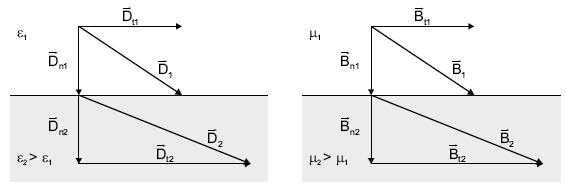
\includegraphics[width=0.75\textwidth]{Abbildungen/Kapitel2/Flussdichten_an_Grenzflaechen.png}
    \caption{Verhalten elektrischer und magnetischer Flussdichtevektoren an Grenzflächen von \mbox{Materialien} unterschiedlicher Dielektrizität bzw. Permeabilität}
    \label{fig:2_Flussdichten_an_Grenzflaechen}
\end{figure}

Beim Materialübergang von Flussdichtevektoren ist festzustellen, dass die Normalkomponenten an der Grenzfläche in beiden Materialien konstant sind (vgl. \Abb \ref{fig:2_Flussdichten_an_Grenzflaechen}) \cite{EM_Schirmung}.  

\begin{equation}
    \vec D_{n1} = \vec D_{n2}
\end{equation}
\begin{equation}
    \vec B_{n1} = \vec B_{n2}
\end{equation}


Aus den vorgestellten Materialgleichungen~\ref{eq:2_Materialgleichung_elektrisches_Feld} und \ref{eq:2_Materialgleichung_magnetisches_Feld} ergibt sich daraus für die Normalkomponenten der Feldstärke bei gleichbleibender Flussdichte zwangsläufig ein Sprung an der Grenzfläche im reziproken Verhältnis der Dielektrizitäten bzw. Permeabilitäten aufgrund der unterschiedlichen Materialeigenschaften. Somit gilt

\begin{equation}
    \vec E_{n1} = \frac{\varepsilon_2}{\varepsilon_1} \cdot \vec E_{n2} \\
\end{equation}
\begin{equation}
    \vec H_{n1} = \frac{\mu_2}{\mu_1} \cdot \vec H_{n2}
\end{equation}

für die Normalkomponenten der Feldstärken. Die Abbildung \ref{fig:2_Feldstaerken_an_Grenzflaechen} verdeutlicht dies. 

\begin{figure}[ht]
    \centering
    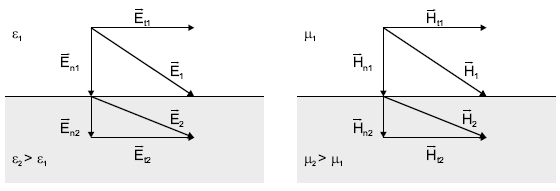
\includegraphics[width=0.75\textwidth]{Abbildungen/Kapitel2/Feldstaerken_an_Grenzflaechen.png}
    \caption{Verhalten elektrischer und magnetischer Feldstärkevektoren an Grenzflächen von \mbox{Materialien} unterschiedlicher Dielektrizität bzw. Permeabilität}
    \label{fig:2_Feldstaerken_an_Grenzflaechen}
\end{figure}

Betrachtet man die Feldursachen bzw. die beschreibenden Maxwell'schen Gleichungen wird offentlichtsicht, dass für die Vektoren der Feldstärke wiederum die Tangentialkomponente in beiden Materialien beim Übergang über die Grenzschicht gleich bleiben muss \cite{EM_Schirmung}. 

\begin{equation}
    \vec E_{t1} = \vec E_{t2}
\end{equation}
\begin{equation}
    \vec H_{t1} = \vec H_{t2}
\end{equation}

Mit einer ähnlichen Argumentation wie vorher kann gezeigt werden, dass damit für die tangentialen Komponenten der Flussdichtevektoren die Beziehungen

\begin{equation}
    \vec D_{t1} = \frac{\varepsilon_1}{\varepsilon_2} \vec D_{t2}
\end{equation}
\begin{equation}
    \vec B_{t1} = \frac{\mu_1}{\mu_2} \vec B_{t2}
\end{equation}

Damit gelten ebenfalls für die resultierenden Vektoren $\vec D_1$ und $\vec D_2$ bzw. $\vec B_1$ und $\vec B_2$ die Materialgesetze~\ref{eq:2_Materialgleichung_elektrisches_Feld} und \ref{eq:2_Materialgleichung_magnetisches_Feld}. Ein Sprung in den Materialeigenschaften äußert sich demnach in einer Brechung der resultierenden Feldlinien in Abhängigkeit der Verhältnisse $\varepsilon_1 / \varepsilon_2$ und $\mu_1 / \mu_2$, welche analog der Brechung von Licht beim Übergang in unterschiedliche optische Materialien veranschaulicht werden kann. Unter der Vorraussetzung isotroper Materialien hintsichtlicht Dielektrizität und Permeabilität gilt weiterhin, dass die resultierenden Flussdichte- und Feldstärkevektoren des elektrischen bzw. magnetischen Feldes in den jeweiligen Materialien kollinear sind und die gleiche Orientierung haben.

\par
\vspace{\linespace}

Für das Verständnis der Wirkungsweise von elektromagnetischen Schirmen ist dieses Verhalten von Feldern an Grenzflächen eine wichtige Grundvoraussetzung.




%Da Schirm für eindringende Wellen -> wichtig








